\chapter{Lösungskonzept}

Das Lösungskonzept beinhaltet die Grundlagen für die erfolgreiche Umsetzung des Prototypen. Der Inhalt ist hauptsächlich aus den Bereich Management und Anforderungen. Die unter Anforderungen aufgenommenen Punkte sind in Zusammenarbeit mit dem Projektpartner entstanden, um so auch die Ansprüche des Forschungsprojektes zu erfüllen.

\section{Projektmanagement}

Führung und Kontrolle des Projekte werden im folgenden Kapitel aufgezeigt. Das Management funktioniert agil, dafür werden geeignete Methoden (vgl. \textit{ScrumDo}) eingesetzt.

\subsection{Projektstrukturplan}
Die \autoref{fig:projektstrukturplan} gewährt einen Überblick über das Projekt. Sie stellt die wichtigsten Bereich und Phasen dar, worin die Arbeit grob eingegliedert werden kann.

\begin{figure}[ht]
\centering
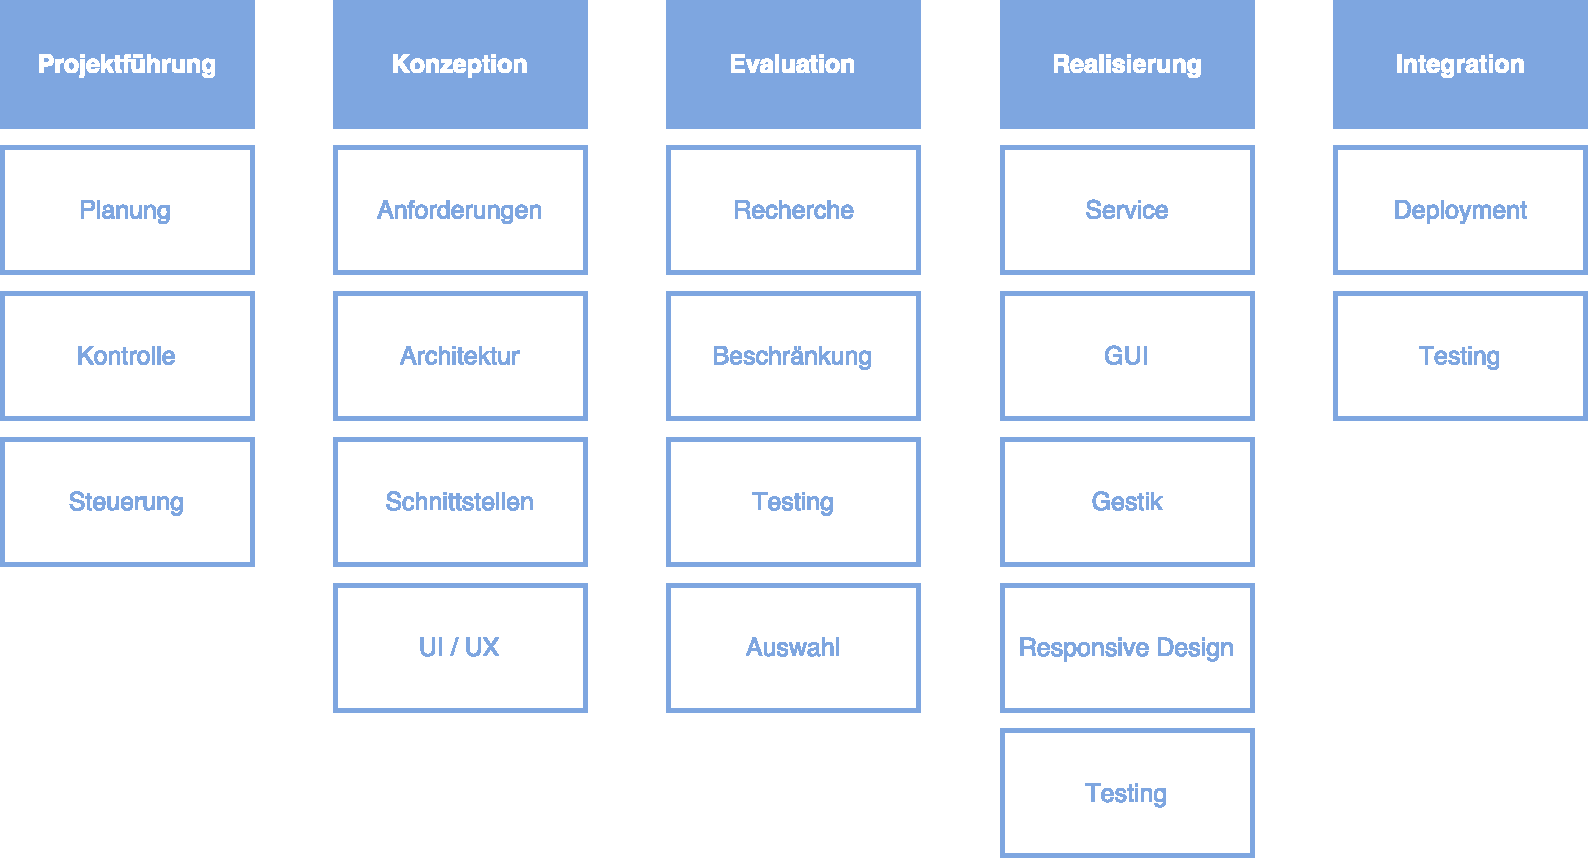
\includegraphics[width=0.7\textwidth]{Projektstrukturplan}
\caption{Projektstrukturplan}
\label{fig:projektstrukturplan}
\end{figure}


\subsection{Projektführung}



\section{Anforderungen}

Für die weitere Unterteilung in Arbeitspakete und Stories, werden die Anforderungen zunächst in Prosa gesammelt. Diese entstammen dem Kundenworkshop und der Aufgabenstellung.

\subsection{Projektmanagement}

\begin{enumerate}
    \item Das Projekt wird agil in allen Bereichen agil geführt.
\end{enumerate}

\subsection{Funktionale Anforderungen}

\begin{table}
  \centering
  \begin{tabular}{|p{1.1cm} | p{1.6cm} | p{8cm}|}
  \hline
    ID & Priorität & Beschreibung \\\hline
    A1.1 & X & Die zugrunde liegende Datenbasis kann mittels eines Graphen visualisiert werden. Jener besteht aus Knoten und Kanten, welche gerichtet und beschriftet sind.\\\hline
    A1.2 & X & Der zu erarbeitende Prototyp kann bidirektional mit dem \textit{ikc-core}-Prototypen interagieren. Änderungen am \textit{ikc-core} sind in der Visualisierung sichtbar. Es ist jedoch es auch möglich Änderungen direkt in der Visualisierung vorzunehmen.\\\hline
    A1.3 & X & Mittels der Visualisierung können die grundlegenden Datenbankoperationen \textit{CREATE}, \textit{READ}, \textit{UPDATE} und \textit{DELETE} (CRUD) direkt auf der Datenbasis des \textit{ikc-core} angewendet werden.\\\hline
    A1.4 & X & Der Prototyp kann auf Smartphones und Tablets benutzt werden.\\\hline
    A1.5 & X & Der Prototyp kann auf Laptops und Desktop-Computern benutzt werden.\\\hline    
    A1.6 & X & Mit Hilfe verschiedener Kriterien (beispielsweise Kontext oder Nachbarschaft) kann ein Teilgraph visualisiert werden.\\\hline 
    A1.61 & X & Diese Teilgraphen (Sichten) können unabhängig von der Datenbasis persistiert werden. Es können, zusätzlich zu den Knoten und Kanten, auch deren relative Positionen in der Visualisierung gespeichert werden.\\\hline 
    A1.7 & X & Der Prototyp kann (unter anderem) mit Drag and Drop bedient werden.\\\hline
    A1.71 & X & Ein mittels Drag and Drop erstellter Knoten kann direkt mit einen im Diagramm bestehenden Knoten verknüft werden. Diese Verknüpfung ist standardmässig bidirektional und unbeschriftet (unlabeled).\\\hline
    A1.72 & X & Ein, im bestehenden User-Interface, mittels der Suche gefundener Knoten kann per Drag and Drop direkt in die Visualisierung übernommen werden.\\\hline 
    A1.8 & X & Die Visualisierung kann innerhalb der bestehenden \textit{ikc-core} Oberfläche genutzt werden.\\\hline 
    A1.9 & X & In der Visualisierung könnnen auch Knoten mit mehr als sieben Kindknoten dargestellt werden. Möglicher Ansatz: Sind mehr als sieben Kindknoten vorhanden, kann anstelle einer Repräsentation jedes einzelnen Knotens auf eine Liste gewechselt werden. Diese Liste kann zusätzlich mit einer Such- und oder Filterfunktion versehen werden.\\\hline     
     
  \end{tabular}
    \caption{Funktionale Anforderungen}
  \label{tab:funktionale-anforderungen}
\end{table}

\subsection{Nicht funktionale Anforderungen}

\begin{table}
  \centering
  \begin{tabular}{|p{0.9cm} | p{1.6cm} | p{8cm}|}
  \hline
    ID & Priorität & Beschreibung \\\hline
    A2.1 & X & Es können Teile des bestehenden \textit{ikc-core} wiederverwendet / erweitert werden (Nachhaltige Entwicklung).\\\hline
    A2.2 & X & Die Visualisierung kann in verschiedenen Projekten wiederverwendet werden.\\\hline
    A2.3 & X & Der Prototyp kann direkt mit dem / in den bestehenden \textit{ikc-core} ausgeliefert werden (Deployment).\\\hline
    A2.4 & X & Die Visualisierung wird in einen \textit{Klon} des bestehenden \textit{ikc-core}-\textit{Repositories} integriert. Ist die Entwicklung abgeschlossen können die beiden Entwicklungsstände \textit{gemerged} werden.\\\hline
    A2.5 & X & Alle Daten werden lediglich auf Dropbox persistiert.\\\hline
    A2.2 & X & Es wird eine intuitive, effiziente Bedienung angestrebt. Ein Mass für die Effizienz: $\frac{\text{Taps}}{\text{Zeit}}$\\\hline
    A2.6 & X & Randbedingungen 180h pro Person\\\hline
    A2.7 & X & Die Arbeit können in einem Arbeitsjournal, mindestens mit Angaben von Datum, Anzahl Stunden, Arbeitsschritt/Thema, nachverfolgt werden.\\\hline
  \end{tabular}
    \caption{Nicht funktionale Anforderungen}
  \label{tab:nicht-funktionale-anforderungen}
\end{table}

\section{Stories}
